\documentclass[12pt,a4paper]{article}

\usepackage[utf8]{inputenc}
\usepackage[T1]{fontenc}
\usepackage[brazil]{babel}
\usepackage{lmodern}
\usepackage[a4paper,margin=2.5cm]{geometry}
\usepackage{amsmath,amssymb}
\usepackage{graphicx}
\usepackage{booktabs}
\usepackage{multirow}
\usepackage{float}
\usepackage{caption}
\usepackage{xcolor}
\usepackage{listings}
\usepackage[hidelinks]{hyperref}

\definecolor{codebg}{RGB}{248,248,248}
\definecolor{codecomment}{RGB}{0,110,0}
\definecolor{codekw}{RGB}{0,0,160}
\definecolor{codestr}{RGB}{160,40,40}

\lstset{
  language=Python,
  basicstyle=\ttfamily\footnotesize,
  backgroundcolor=\color{codebg},
  keywordstyle=\color{codekw}\bfseries,
  commentstyle=\color{codecomment}\itshape,
  stringstyle=\color{codestr},
  numbers=left,
  numberstyle=\tiny\color{gray},
  frame=single,
  breaklines=true,
  showstringspaces=false,
  tabsize=4,
  inputencoding=utf8,
  extendedchars=true,
  literate=
    {á}{{\'a}}1 {à}{{\`a}}1 {ã}{{\~a}}1 {â}{{\^a}}1
    {é}{{\'e}}1 {ê}{{\^e}}1 {í}{{\'i}}1
    {ó}{{\'o}}1 {õ}{{\~o}}1 {ô}{{\^o}}1
    {ú}{{\'u}}1 {ç}{{\c{c}}}1
    {Á}{{\'A}}1 {É}{{\'E}}1 {Í}{{\'I}}1 {Ó}{{\'O}}1 {Ú}{{\'U}}1 {Ç}{{\c{C}}}1
}

% Link do repositório do código
\newcommand{\repositorio}{\url{https://github.com/juliaPamplona/teia-laboratorios/tree/main/lab4}}

\newcommand{\setosa}{\emph{setosa}}
\newcommand{\versicolor}{\emph{versicolor}}
\newcommand{\virginica}{\emph{virginica}}

\begin{document}

%=====================================================================
% Capa
%=====================================================================
\begin{titlepage}
\centering

\includegraphics[width=0.35\textwidth]{figuras/logo_uepb.png}\\[1.5em]
{\large \textsc{Universidade Estadual da Paraíba}}\\[0.3em]
{\normalsize Disciplina: Tópicos Especiais em Inteligência Artificial}\\[0.3em]
{\normalsize Prof. Robson Pequeno de Sousa}

\vfill

{\LARGE \textbf{Classificador ótimo de Bayes e Naive Bayes aplicados à base Iris}}\\[1em]
{\large Relatório do Laboratório 04 --- Classificação pelo máximo a posteriori com densidades normais}

\vfill

{\large Júlia Pamplona}

\vfill

{\large Novembro de 2026}
\end{titlepage}

%=====================================================================
% Resumo
%=====================================================================
\begin{abstract}
Este relatório descreve a implementação, em Python e sem bibliotecas de aprendizado de máquina, do classificador ótimo de Bayes e do Naive Bayes, ambos com densidades normais e regra de decisão pelo máximo a posteriori (MAP), aplicados às três espécies da base Iris. Antes da classificação, a aderência de cada classe à distribuição normal multivariada foi verificada pelos testes de Henze-Zirkler e de Mardia, no R (pacote MVN) e em uma implementação própria em Python, que reproduziu os p-valores do R. \versicolor{} ($p = 0{,}226$) e \virginica{} ($p = 0{,}497$) são compatíveis com a normal multivariada; a \setosa{} é um caso limítrofe, rejeitada pelo Henze-Zirkler por margem mínima ($p = 0{,}04995$) e aceita pelos testes de assimetria e curtose de Mardia. Com 70\% das amostras para treinamento e 30\% para teste, o classificador ótimo de Bayes acertou as 45 amostras de teste (Kappa $= 1$), e o Naive Bayes errou uma ($A_g = 97{,}78\%$, Kappa $= 0{,}967$). As superfícies de decisão dos três pares de classes foram determinadas analiticamente; são quádricas nos quatro atributos. Pelo teste de significância do Kappa ($Z = 1{,}01$, $p = 0{,}31$), a maior acurácia do classificador ótimo de Bayes não é estatisticamente significativa ao nível de 5\%.

\vspace{1em}
\noindent\textbf{Palavras-chave:} classificador de Bayes; Naive Bayes; máximo a posteriori; normal multivariada; Henze-Zirkler; Mardia; superfície de decisão; coeficiente Kappa; base Iris.
\end{abstract}
\thispagestyle{empty}
\newpage

%=====================================================================
% Sumário
%=====================================================================
\tableofcontents
\thispagestyle{empty}
\newpage

%=====================================================================
\section{Introdução}
%=====================================================================

Nos laboratórios anteriores, as fronteiras de decisão foram obtidas a partir das médias das classes (distância mínima e funções de decisão) ou estimadas iterativamente (perceptron e regra delta). Em todos os casos, eram fronteiras lineares. Neste laboratório, a decisão passa a ser probabilística: cada classe é descrita por uma densidade de probabilidade, e o padrão é atribuído à classe mais provável dada a observação. Com densidades normais e matrizes de covariância diferentes entre as classes, as fronteiras resultantes são quadráticas.

Os objetivos, definidos no enunciado, são:
\begin{enumerate}
  \setcounter{enumi}{-1}
  \item verificar, para cada classe, a aderência à normal multivariada pelos testes de Henze-Zirkler e de Mardia;
  \item[a)] usar 70\% dos dados para treinamento e 30\% para teste;
  \item[b)] classificar as três classes pelo máximo a posteriori (MAP), com o classificador ótimo de Bayes e com o Naive Bayes, supondo probabilidades a priori iguais;
  \item[c)] determinar as superfícies de decisão de \setosa{}~$\times$~\virginica{}, \versicolor{}~$\times$~\virginica{} e \setosa{}~$\times$~\versicolor{};
  \item[d)] determinar, em todos os casos, a matriz de confusão e as métricas de qualidade estudadas;
  \item[e)] decidir qual classificador tem maior acurácia, usando o teste de significância do Kappa.
\end{enumerate}

%=====================================================================
\section{Fundamentação teórica}\label{sec:teoria}
%=====================================================================

\subsection{Classificação pelo máximo a posteriori}

Pelo teorema de Bayes, a probabilidade a posteriori da classe $C_j$ dada a observação $\mathbf{x}$ é
\begin{equation}
  P(C_j \mid \mathbf{x}) = \frac{P(\mathbf{x} \mid C_j)\,P(C_j)}{P(\mathbf{x})}.
  \label{eq:bayes}
\end{equation}
O classificador MAP atribui $\mathbf{x}$ à classe de maior probabilidade a posteriori. Como $P(\mathbf{x})$ é igual para todas as classes e, neste laboratório, as probabilidades a priori também são iguais, $P(C_1) = P(C_2) = P(C_3)$, os dois termos podem ser suprimidos, e a decisão depende apenas da verossimilhança:
\begin{equation}
  C^* = \arg\max_j P(C_j \mid \mathbf{x}) = \arg\max_j P(\mathbf{x} \mid C_j).
  \label{eq:map}
\end{equation}
Esse é o classificador que minimiza a probabilidade de erro, por isso é chamado de classificador ótimo de Bayes.

\subsection{Classificador ótimo de Bayes com densidade normal}

Verificada a normalidade dos dados, a densidade de cada classe é a normal multivariada de vetor de médias $\mathbf{m}_j$ e matriz de covariância $\boldsymbol{\Sigma}_j$:
\begin{equation}
  P(\mathbf{x} \mid C_j) = \frac{1}{(2\pi)^{n/2}|\boldsymbol{\Sigma}_j|^{1/2}}
  \exp\left[-\frac{1}{2}(\mathbf{x} - \mathbf{m}_j)^t\boldsymbol{\Sigma}_j^{-1}(\mathbf{x} - \mathbf{m}_j)\right].
  \label{eq:normal}
\end{equation}
Como o logaritmo é crescente, maximizar $P(\mathbf{x} \mid C_j)$ equivale a maximizar seu logaritmo. Descartando o termo $-\frac{n}{2}\ln 2\pi$, comum a todas as classes, a função discriminante é
\begin{equation}
  g_j(\mathbf{x}) = -\frac{1}{2}\ln|\boldsymbol{\Sigma}_j| - \frac{1}{2}(\mathbf{x} - \mathbf{m}_j)^t\boldsymbol{\Sigma}_j^{-1}(\mathbf{x} - \mathbf{m}_j),
  \label{eq:g_bayes}
\end{equation}
em que o segundo termo é a distância de Mahalanobis ao quadrado entre $\mathbf{x}$ e $\mathbf{m}_j$, com sinal negativo. Os parâmetros são estimados no conjunto de treinamento por máxima verossimilhança:
\begin{equation}
  \mathbf{m}_j = \frac{1}{N_j}\sum_{\mathbf{x} \in C_j}\mathbf{x}, \qquad
  \boldsymbol{\Sigma}_j = \frac{1}{N_j}\sum_{\mathbf{x} \in C_j}(\mathbf{x} - \mathbf{m}_j)(\mathbf{x} - \mathbf{m}_j)^t.
  \label{eq:estimativas}
\end{equation}

\subsection{Naive Bayes}

O Naive Bayes supõe que os atributos são condicionalmente independentes dentro de cada classe, de modo que a densidade conjunta é o produto das densidades univariadas:
\begin{equation}
  P(\mathbf{x} \mid C_j) = \prod_{k=1}^{n} P(x_k \mid C_j), \qquad
  P(x_k \mid C_j) = \frac{1}{\sqrt{2\pi s_{jk}^2}}\exp\left[-\frac{(x_k - m_{jk})^2}{2 s_{jk}^2}\right].
  \label{eq:naive}
\end{equation}
É o caso particular da Eq.~\eqref{eq:normal} com $\boldsymbol{\Sigma}_j$ diagonal, e a função discriminante fica
\begin{equation}
  g_j(\mathbf{x}) = -\frac{1}{2}\sum_{k=1}^{n}\left[\ln s_{jk}^2 + \frac{(x_k - m_{jk})^2}{s_{jk}^2}\right].
  \label{eq:g_naive}
\end{equation}
O Naive Bayes estima $2n$ parâmetros por classe (médias e variâncias), contra $n + n(n+1)/2$ do classificador completo, mas ignora as correlações entre os atributos.

\subsection{Superfície de decisão}\label{sec:superficie_teoria}

A superfície de decisão entre as classes $C_i$ e $C_j$ é o conjunto de pontos em que as duas funções discriminantes são iguais, $d_{ij}(\mathbf{x}) = g_i(\mathbf{x}) - g_j(\mathbf{x}) = 0$. Expandindo a Eq.~\eqref{eq:g_bayes} com $\mathbf{P}_j = \boldsymbol{\Sigma}_j^{-1}$, obtém-se a forma quadrática
\begin{equation}
  d_{ij}(\mathbf{x}) = \mathbf{x}^t\mathbf{A}\,\mathbf{x} + \mathbf{b}^t\mathbf{x} + c = 0,
  \label{eq:superficie}
\end{equation}
com
\begin{equation}
  \mathbf{A} = -\frac{1}{2}(\mathbf{P}_i - \mathbf{P}_j), \quad
  \mathbf{b} = \mathbf{P}_i\mathbf{m}_i - \mathbf{P}_j\mathbf{m}_j, \quad
  c = -\frac{1}{2}\left(\mathbf{m}_i^t\mathbf{P}_i\mathbf{m}_i - \mathbf{m}_j^t\mathbf{P}_j\mathbf{m}_j\right) - \frac{1}{2}\ln\frac{|\boldsymbol{\Sigma}_i|}{|\boldsymbol{\Sigma}_j|}.
  \label{eq:coeficientes}
\end{equation}
$d_{ij}(\mathbf{x}) > 0$ indica a classe $C_i$, e $d_{ij}(\mathbf{x}) < 0$, a classe $C_j$. Como $\boldsymbol{\Sigma}_i \ne \boldsymbol{\Sigma}_j$, a matriz $\mathbf{A}$ não se anula e a superfície é uma quádrica (hiperquádrica em quatro dimensões). Só quando as covariâncias são iguais o termo quadrático desaparece e a fronteira volta a ser um hiperplano. No Naive Bayes, $\mathbf{A}$ é diagonal: a superfície também é quadrática, mas sem termos cruzados $x_k x_l$.

\subsection{Testes de normalidade multivariada}\label{sec:testes_normalidade}

Nos dois testes, a hipótese nula é $H_0$: os dados vêm de uma população normal multivariada; se $p > 0{,}05$, $H_0$ não é rejeitada. Sejam $n$ amostras com $p$ atributos, média $\bar{\mathbf{x}}$ e covariância de máxima verossimilhança $\mathbf{S}$, e as distâncias de Mahalanobis ao quadrado
\begin{equation}
  D_i = (\mathbf{x}_i - \bar{\mathbf{x}})^t\mathbf{S}^{-1}(\mathbf{x}_i - \bar{\mathbf{x}}), \qquad
  D_{ik} = (\mathbf{x}_i - \mathbf{x}_k)^t\mathbf{S}^{-1}(\mathbf{x}_i - \mathbf{x}_k).
\end{equation}

\paragraph{Henze-Zirkler.} O teste compara a função característica empírica, ponderada, com a da normal~\cite{henze}:
\begin{equation}
  HZ = n\left[\frac{1}{n^2}\sum_{i=1}^{n}\sum_{k=1}^{n} e^{-\frac{\beta^2}{2}D_{ik}}
  - \frac{2}{(1+\beta^2)^{p/2}}\,\frac{1}{n}\sum_{i=1}^{n} e^{-\frac{\beta^2}{2(1+\beta^2)}D_i}
  + \frac{1}{(1+2\beta^2)^{p/2}}\right],
  \label{eq:hz}
\end{equation}
com $\beta = \frac{1}{\sqrt{2}}\left(\frac{2p+1}{4}\right)^{1/(p+4)} n^{1/(p+4)}$. Sob $H_0$, $HZ$ segue aproximadamente uma distribuição log-normal, de onde vem o p-valor.

\paragraph{Mardia.} O teste avalia separadamente a assimetria e a curtose multivariadas~\cite{mardia}:
\begin{equation}
  b_{1} = \frac{1}{n^2}\sum_{i=1}^{n}\sum_{k=1}^{n}\left[(\mathbf{x}_i - \bar{\mathbf{x}})^t\mathbf{S}^{-1}(\mathbf{x}_k - \bar{\mathbf{x}})\right]^3, \qquad
  b_{2} = \frac{1}{n}\sum_{i=1}^{n} D_i^2.
  \label{eq:mardia}
\end{equation}
Sob $H_0$, $n b_1/6 \sim \chi^2$ com $p(p+1)(p+2)/6$ graus de liberdade (20, para $p = 4$), e $(b_2 - p(p+2))/\sqrt{8p(p+2)/n} \sim N(0,1)$. Os dados são considerados normais quando os dois p-valores são maiores que 0,05.

\paragraph{Gráfico Q-Q de qui-quadrado.} Sob normalidade, as distâncias $D_i$ seguem aproximadamente uma $\chi^2$ com $p$ graus de liberdade. O gráfico das $D_i$ ordenadas contra os quantis da $\chi^2_p$ deve ficar próximo da reta identidade.

\subsection{Métricas de qualidade}

As métricas são as da aula PR51, já implementadas no Laboratório~03. A matriz de confusão tem as linhas para a predição e as colunas para a referência; dela se extraem o acerto global $A_g$, as acurácias do produtor $A_{pi} = a_{ii}/a_{+i}$ (sensibilidade) e do usuário $A_{ui} = a_{ii}/a_{i+}$ (precisão), os coeficientes Kappa e Tau com suas variâncias e, para cada classe tomada contra as demais, a especificidade, $F_1$, $F_2$ e o coeficiente de Matthews (MCC). Dois classificadores são comparados pela estatística
\begin{equation}
  Z = \frac{k_1 - k_2}{\sqrt{\sigma_1^2 + \sigma_2^2}} \sim N(0, 1),
  \label{eq:z}
\end{equation}
rejeitando-se $H_0$ (não há diferença) ao nível de 5\% se $|Z| > 1{,}96$.

%=====================================================================
\section{Base de dados}
%=====================================================================

A base Iris (arquivo \texttt{Iris data.xls}) contém 150 amostras, 50 de cada espécie: \setosa{}, \versicolor{} e \virginica{}. Cada amostra é descrita pelo vetor de características $\mathbf{x} = (x_1, x_2, x_3, x_4)^t$ da Tabela~\ref{tab:atributos}.

\begin{table}[H]
\centering
\caption{Atributos da base Iris na ordem do arquivo.}
\label{tab:atributos}
\begin{tabular}{cll}
\toprule
Atributo & Coluna & Descrição \\
\midrule
$x_1$ & \texttt{Sepal length} & comprimento da sépala (cm) \\
$x_2$ & \texttt{Sepal width}  & largura da sépala (cm) \\
$x_3$ & \texttt{Petal length} & comprimento da pétala (cm) \\
$x_4$ & \texttt{Petal width}  & largura da pétala (cm) \\
\bottomrule
\end{tabular}
\end{table}

%=====================================================================
\section{Metodologia e implementação}
%=====================================================================

Os classificadores, as métricas e os testes de normalidade foram implementados em Python, usando apenas \texttt{pandas} (leitura da planilha), \texttt{numpy} (álgebra linear) e \texttt{matplotlib} (gráficos). Os testes de normalidade também foram executados no R~4.6.2 com o pacote MVN~6.3~\cite{mvn}. O código-fonte e as figuras estão disponíveis no repositório \repositorio.

\subsection{Organização do sistema}

\begin{table}[H]
\centering
\caption{Módulos do Laboratório 04.}
\label{tab:modulos}
\begin{tabular}{lp{10.5cm}}
\toprule
Arquivo & Responsabilidade \\
\midrule
\texttt{dados.py}          & leitura da Iris e divisão estratificada 70/30 \\
\texttt{normalidade.py}    & testes de Henze-Zirkler e Mardia em NumPy \\
\texttt{normalidade.R}     & os mesmos testes com o pacote MVN e os gráficos Q-Q \\
\texttt{bayes.py}          & classificador ótimo de Bayes, Naive Bayes, regra MAP e superfícies de decisão \\
\texttt{metricas.py}       & matriz de confusão e métricas da aula PR51 \\
\texttt{visualizacao.py}   & impressões no terminal e gráficos \\
\texttt{lab4\_bayes.py}    & execução de todos os itens e conclusões \\
\bottomrule
\end{tabular}
\end{table}

\subsection{Verificação da normalidade}

Os testes foram aplicados às 50 amostras de cada classe, com os quatro atributos. No R, o script \texttt{normalidade.R} usa as funções \texttt{mvn}, \texttt{hz} e \texttt{mardia} do pacote MVN. A tabela produzida por \texttt{mvn} arredonda o p-valor para três casas, o que esconde o resultado da \setosa{}; por isso o script também imprime os valores completos das funções \texttt{hz} e \texttt{mardia}. Em Python, as Eqs.~\eqref{eq:hz} e~\eqref{eq:mardia} foram implementadas à mão, com as distribuições log-normal, normal e $\chi^2$ calculadas pelas funções \texttt{math.erfc} e \texttt{math.lgamma}, e reproduziram os p-valores do R até a sexta casa decimal.

\subsection{Divisão 70\% / 30\%}

A divisão é estratificada: as 50 amostras de cada espécie são embaralhadas (semente 42) e separadas em 35 para treinamento e 15 para teste, totalizando 105 e 45 amostras. Não há conjunto de validação.

\subsection{Classificadores}

Os parâmetros da Eq.~\eqref{eq:estimativas} são calculados no treinamento. A função discriminante do classificador ótimo de Bayes calcula a distância de Mahalanobis resolvendo o sistema linear $\boldsymbol{\Sigma}_j\mathbf{z} = \mathbf{x} - \mathbf{m}_j$, sem inverter a matriz explicitamente, e usa o logaritmo do determinante calculado por \texttt{np.linalg.slogdet}, que é numericamente estável:

\begin{lstlisting}[title=\texttt{bayes.py} --- função discriminante do classificador ótimo de Bayes]
def pontuar_bayes_gaussiano(X_amostras, parametros):
    X_amostras = np.atleast_2d(np.asarray(X_amostras, dtype=float))
    diferencas = X_amostras - parametros["media"]

    # Distância de Mahalanobis ao quadrado, sem inverter Sigma
    resolvido = np.linalg.solve(parametros["covariancia"], diferencas.T).T
    mahalanobis = np.sum(diferencas * resolvido, axis=1)

    return -0.5 * (parametros["logdet"] + mahalanobis)
\end{lstlisting}

A regra MAP da Eq.~\eqref{eq:map} escolhe a classe de maior $g_j(\mathbf{x})$. Para avaliar os pares de classes do item~(c), a mesma regra é aplicada restringindo a decisão às duas classes do par e usando apenas as amostras de teste dessas classes.

\subsection{Superfícies de decisão}

Os coeficientes $\mathbf{A}$, $\mathbf{b}$ e $c$ da Eq.~\eqref{eq:coeficientes} são calculados para cada par e cada classificador. Para conferir a expansão algébrica, o código verifica que $\mathbf{x}^t\mathbf{A}\mathbf{x} + \mathbf{b}^t\mathbf{x} + c$ coincide com $g_i(\mathbf{x}) - g_j(\mathbf{x})$ em todas as amostras de teste.

Uma superfície em quatro dimensões não pode ser desenhada diretamente. Para os gráficos, o classificador continua usando os quatro atributos, mas a superfície é cortada no plano da pétala $(x_3, x_4)$, com a sépala $(x_1, x_2)$ fixa na média do treinamento das duas classes do par. Com $\mathbf{x} = (\mathbf{f}, \mathbf{u})$, em que $\mathbf{f}$ são os atributos fixos e $\mathbf{u}$ os visualizados, a fatia é a cônica
\begin{equation}
  d(\mathbf{u}) = \mathbf{u}^t\mathbf{A}_{uu}\mathbf{u} + (\mathbf{b}_u + 2\mathbf{A}_{uf}\mathbf{f})^t\mathbf{u} + (c + \mathbf{b}_f^t\mathbf{f} + \mathbf{f}^t\mathbf{A}_{ff}\mathbf{f}) = 0.
  \label{eq:fatia}
\end{equation}

%=====================================================================
\section{Resultados}\label{sec:resultados}
%=====================================================================

\subsection{Normalidade multivariada}

A Tabela~\ref{tab:normalidade} reúne os resultados, que coincidem no R e em Python.

\begin{table}[H]
\centering
\caption{Testes de normalidade multivariada por classe ($n = 50$, $p = 4$).}
\label{tab:normalidade}
\small
\begin{tabular}{lcccccccc}
\toprule
 & \multicolumn{2}{c}{Henze-Zirkler} & \multicolumn{2}{c}{Mardia: assimetria} & \multicolumn{2}{c}{Mardia: curtose} & \multicolumn{2}{c}{Veredito} \\
\cmidrule(lr){2-3}\cmidrule(lr){4-5}\cmidrule(lr){6-7}\cmidrule(lr){8-9}
Classe & $HZ$ & $p$ & Estat. & $p$ & Estat. & $p$ & HZ & Mardia \\
\midrule
\setosa{}     & 0,9488 & 0,04995 & 25,664 & 0,1772 & 1,295     & 0,1953 & não normal & normal \\
\versicolor{} & 0,8388 & 0,2262  & 25,185 & 0,1944 & $-0{,}572$ & 0,5674 & normal & normal \\
\virginica{}  & 0,7570 & 0,4970  & 26,271 & 0,1571 & 0,153     & 0,8787 & normal & normal \\
\bottomrule
\end{tabular}
\end{table}

\versicolor{} e \virginica{} passam nos dois testes, com p-valores bem acima de 0,05. A \setosa{} é um caso limítrofe: o Henze-Zirkler dá $p = 0{,}049954$. A tabela do MVN exibe esse valor como ``0,05'', mas o valor completo, conferido no R e em Python, é menor que 0,05, e $H_0$ é rejeitada por margem mínima. Os testes de Mardia não acusam desvio de assimetria ($p = 0{,}177$) nem de curtose ($p = 0{,}195$). No gráfico Q-Q (Figura~\ref{fig:qq}), os pontos da \setosa{} acompanham a reta até cerca de $\chi^2 = 6$ e se afastam um pouco dela na cauda superior, sem desvio acentuado.

\begin{figure}[H]
\centering
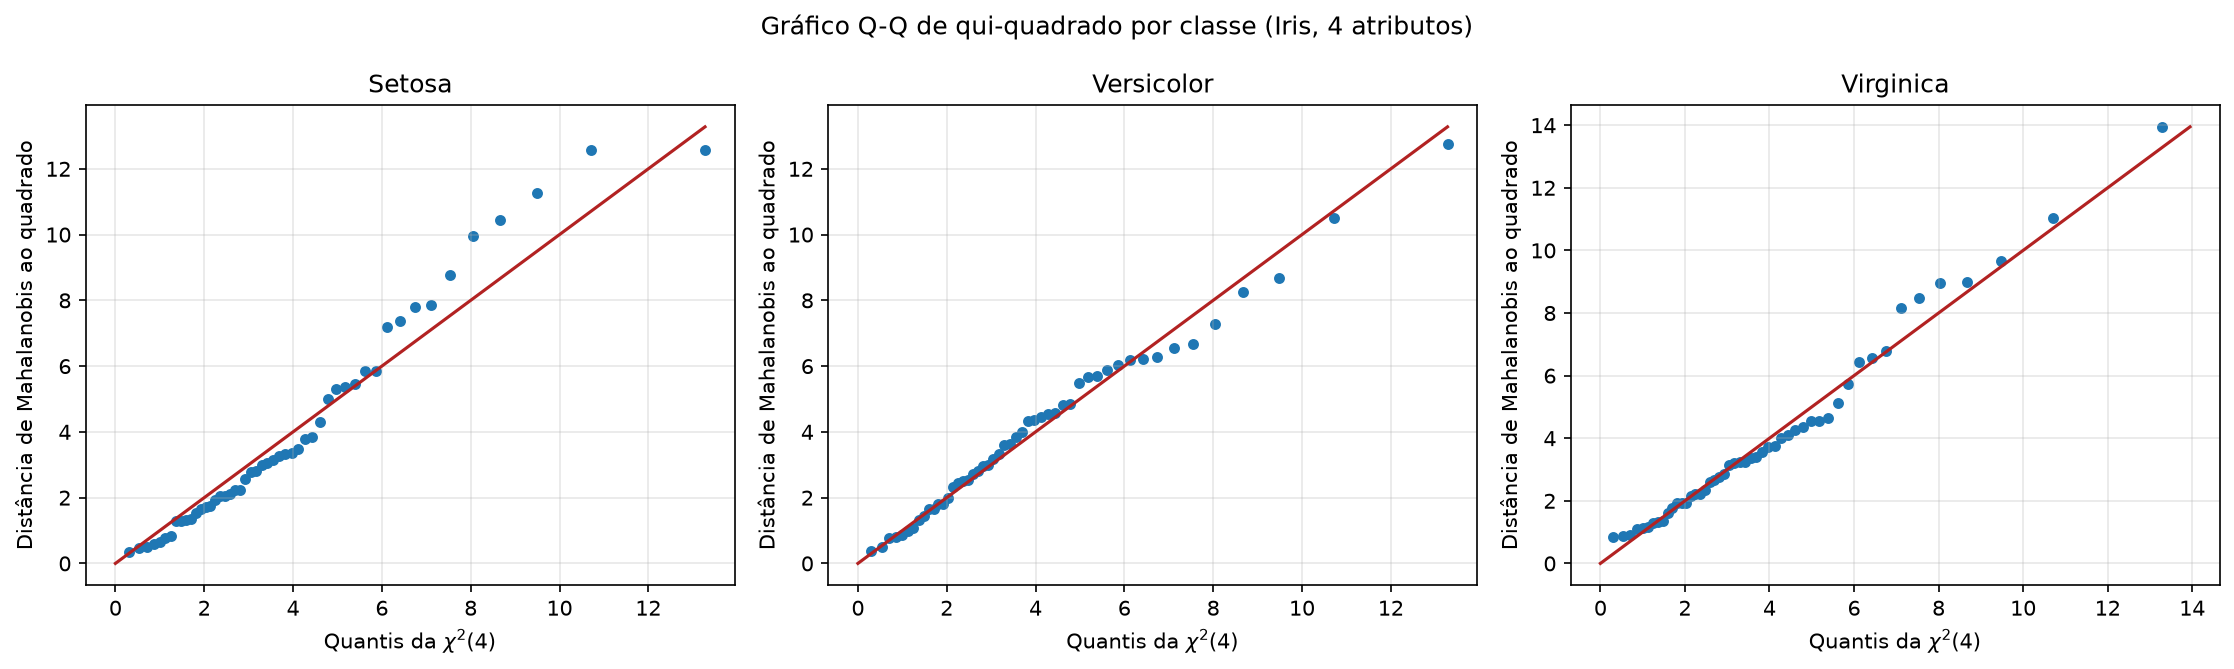
\includegraphics[width=\textwidth]{figuras/qq_quiquadrado.png}
\caption{Gráfico Q-Q de qui-quadrado das distâncias de Mahalanobis de cada classe.}
\label{fig:qq}
\end{figure}

Com isso, a hipótese de normalidade foi adotada para as três classes, com a ressalva de que, para a \setosa{}, ela é apenas aproximada. A ressalva não compromete a classificação, porque a \setosa{} é separada sem erro das outras duas espécies em todos os experimentos.

\subsection{Parâmetros estimados}

\begin{table}[H]
\centering
\caption{Vetores de médias $\mathbf{m}_j$ estimados no treinamento (35 amostras por classe).}
\label{tab:medias}
\begin{tabular}{lcccc}
\toprule
Classe & $x_1$ & $x_2$ & $x_3$ & $x_4$ \\
\midrule
\setosa{}     & 5,0257 & 3,4286 & 1,5143 & 0,2657 \\
\versicolor{} & 5,9771 & 2,8257 & 4,3086 & 1,3743 \\
\virginica{}  & 6,6114 & 2,9943 & 5,5686 & 1,9971 \\
\bottomrule
\end{tabular}
\end{table}

As matrizes de covariância do classificador ótimo de Bayes são
\begin{gather*}
\boldsymbol{\Sigma}_{\text{set}} = \begin{pmatrix}0{,}0991 & 0{,}0884 & 0{,}0151 & 0{,}0115 \\ 0{,}0884 & 0{,}1409 & 0{,}0144 & 0{,}0096 \\ 0{,}0151 & 0{,}0144 & 0{,}0229 & 0{,}0039 \\ 0{,}0115 & 0{,}0096 & 0{,}0039 & 0{,}0131\end{pmatrix}, \quad
\boldsymbol{\Sigma}_{\text{ver}} = \begin{pmatrix}0{,}2915 & 0{,}0820 & 0{,}1913 & 0{,}0503 \\ 0{,}0820 & 0{,}0893 & 0{,}0786 & 0{,}0347 \\ 0{,}1913 & 0{,}0786 & 0{,}2282 & 0{,}0682 \\ 0{,}0503 & 0{,}0347 & 0{,}0682 & 0{,}0333\end{pmatrix}, \\[0.5em]
\boldsymbol{\Sigma}_{\text{vir}} = \begin{pmatrix}0{,}3570 & 0{,}0981 & 0{,}2629 & 0{,}0283 \\ 0{,}0981 & 0{,}0903 & 0{,}0744 & 0{,}0386 \\ 0{,}2629 & 0{,}0744 & 0{,}2479 & 0{,}0233 \\ 0{,}0283 & 0{,}0386 & 0{,}0233 & 0{,}0717\end{pmatrix}.
\end{gather*}
O Naive Bayes usa apenas as diagonais dessas matrizes. As covariâncias fora da diagonal não são desprezíveis: na \versicolor{}, por exemplo, a covariância entre o comprimento da sépala e o da pétala (0,1913) corresponde a uma correlação de 0,74. É essa informação que o Naive Bayes descarta.

\subsection{Classificação das três classes}

\begin{table}[H]
\centering
\caption{Matrizes de confusão no conjunto de teste (linhas: predição; colunas: referência).}
\label{tab:mc3}
\begin{tabular}{l|ccc||l|ccc}
\toprule
Bayes ótimo & Set. & Ver. & Vir. & Naive Bayes & Set. & Ver. & Vir. \\
\midrule
\setosa{}     & 15 & 0  & 0  & \setosa{}     & 15 & 0  & 0  \\
\versicolor{} & 0  & 15 & 0  & \versicolor{} & 0  & 15 & 1  \\
\virginica{}  & 0  & 0  & 15 & \virginica{}  & 0  & 0  & 14 \\
\bottomrule
\end{tabular}
\end{table}

\begin{figure}[H]
\centering
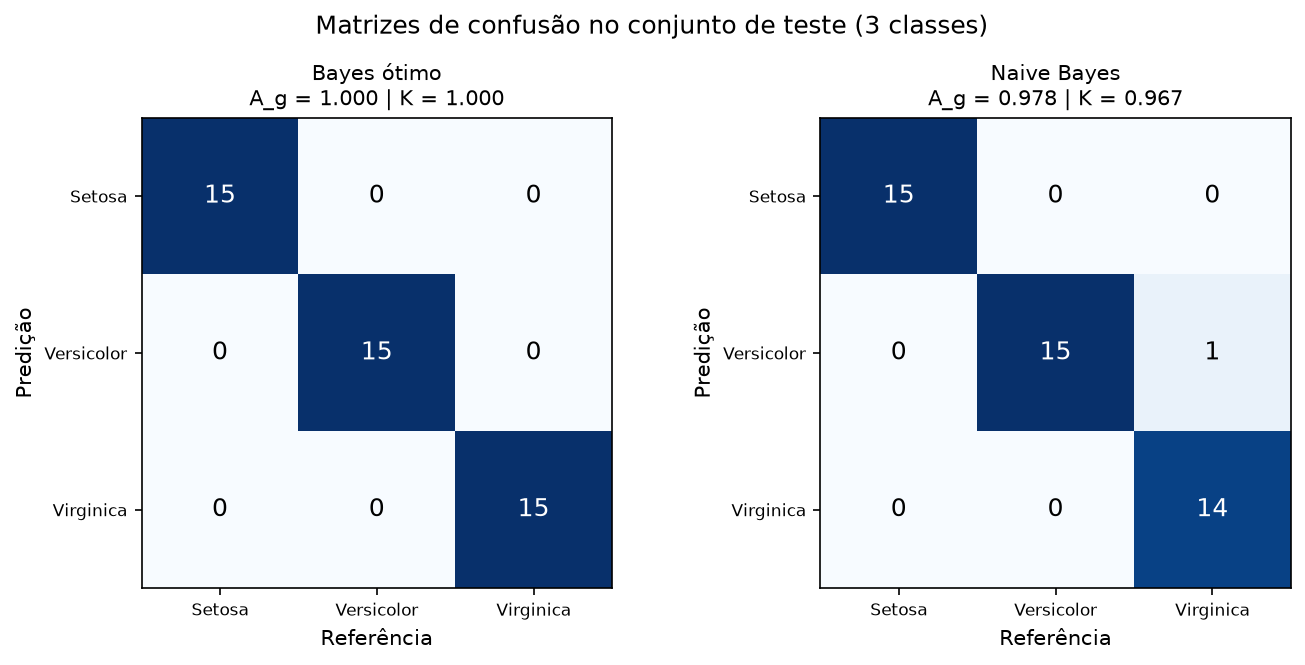
\includegraphics[width=0.75\textwidth]{figuras/matrizes_confusao.png}
\caption{Matrizes de confusão dos dois classificadores nas três classes.}
\label{fig:matrizes}
\end{figure}

\begin{table}[H]
\centering
\caption{Métricas multiclasse no conjunto de teste ($m = 45$, $C = 3$).}
\label{tab:metricas3}
\begin{tabular}{lcccccc}
\toprule
Classificador & $A_g$ & $A_a$ & $K$ & $\sigma_K^2$ & $\tau$ & $\sigma_\tau^2$ \\
\midrule
Bayes ótimo & 1,0000 & 0,3333 & 1,0000 & 0,000000 & 1,0000 & 0,000000 \\
Naive Bayes & 0,9778 & 0,3333 & 0,9667 & 0,001085 & 0,9667 & 0,001086 \\
\bottomrule
\end{tabular}
\end{table}

\begin{table}[H]
\centering
\caption{Métricas por classe (classe $\times$ resto) no conjunto de teste.}
\label{tab:binarias3}
\small
\begin{tabular}{llcccccc}
\toprule
Classificador & Classe & $A_p$ & $A_u$ & Espec. & $F_1$ & $F_2$ & MCC \\
\midrule
\multirow{3}{*}{Bayes ótimo}
 & \setosa{}     & 1,0000 & 1,0000 & 1,0000 & 1,0000 & 1,0000 & 1,0000 \\
 & \versicolor{} & 1,0000 & 1,0000 & 1,0000 & 1,0000 & 1,0000 & 1,0000 \\
 & \virginica{}  & 1,0000 & 1,0000 & 1,0000 & 1,0000 & 1,0000 & 1,0000 \\
\midrule
\multirow{3}{*}{Naive Bayes}
 & \setosa{}     & 1,0000 & 1,0000 & 1,0000 & 1,0000 & 1,0000 & 1,0000 \\
 & \versicolor{} & 1,0000 & 0,9375 & 0,9667 & 0,9677 & 0,9868 & 0,9520 \\
 & \virginica{}  & 0,9333 & 1,0000 & 1,0000 & 0,9655 & 0,9459 & 0,9504 \\
\bottomrule
\end{tabular}
\end{table}

O classificador ótimo de Bayes acertou as 45 amostras de teste. O Naive Bayes errou uma \virginica{}, classificada como \versicolor{}; por isso, a acurácia do produtor da \virginica{} e a do usuário da \versicolor{} caem para 0,9333 e 0,9375. Kappa e Tau coincidem porque o teste é balanceado (15 amostras por classe), o que faz o acerto casual valer exatamente $1/C$.

\subsection{Superfícies de decisão}\label{sec:superficies}

As equações a seguir são as superfícies $d_{ij}(\mathbf{x}) = 0$ da Eq.~\eqref{eq:superficie}, com os quatro atributos. Em cada par, $d_{ij}(\mathbf{x}) > 0$ indica a primeira classe e $d_{ij}(\mathbf{x}) < 0$, a segunda.

\paragraph{(i) \setosa{} $\times$ \virginica{}.} Classificador ótimo de Bayes:
{\small
\begin{multline*}
 - 5{,}5358\,x_1^2 + 1{,}9898\,x_2^2 - 15{,}4812\,x_3^2 - 34{,}1218\,x_4^2 + 9{,}8779\,x_1x_2 \\
 - 7{,}8109\,x_1x_3 + 10{,}9347\,x_1x_4 + 0{,}5044\,x_2x_3 - 9{,}9952\,x_2x_4 + 8{,}6990\,x_3x_4 \\
 + 59{,}0067\,x_1 - 28{,}4281\,x_2 + 29{,}1939\,x_3 - 51{,}5575\,x_4 - 72{,}7378 = 0
\end{multline*}}
Naive Bayes:
{\small
\begin{multline*}
 - 3{,}6473\,x_1^2 + 1{,}9913\,x_2^2 - 19{,}7800\,x_3^2 - 31{,}1653\,x_4^2 \\
 + 32{,}2188\,x_1 - 8{,}8428\,x_2 + 43{,}5485\,x_3 - 7{,}5840\,x_4 - 18{,}1774 = 0
\end{multline*}}

\paragraph{(ii) \versicolor{} $\times$ \virginica{}.} Classificador ótimo de Bayes:
{\small
\begin{multline*}
 2{,}6930\,x_1^2 - 0{,}1746\,x_2^2 - 0{,}3924\,x_3^2 - 39{,}8966\,x_4^2 - 0{,}9839\,x_1x_2 \\
 - 5{,}3167\,x_1x_3 - 6{,}2413\,x_1x_4 - 2{,}1575\,x_2x_3 + 10{,}6423\,x_2x_4 + 28{,}4831\,x_3x_4 \\
 + 10{,}1712\,x_1 + 7{,}0676\,x_2 - 12{,}2634\,x_3 - 16{,}0087\,x_4 + 12{,}8194 = 0
\end{multline*}}
Naive Bayes:
{\small
\begin{multline*}
 - 0{,}3149\,x_1^2 - 0{,}0567\,x_2^2 - 0{,}1738\,x_3^2 - 8{,}0246\,x_4^2 \\
 + 1{,}9876\,x_1 - 1{,}5474\,x_2 - 3{,}5861\,x_3 + 13{,}3701\,x_4 + 26{,}8118 = 0
\end{multline*}}

\paragraph{(iii) \setosa{} $\times$ \versicolor{}.} Classificador ótimo de Bayes:
{\small
\begin{multline*}
 - 8{,}2288\,x_1^2 + 2{,}1644\,x_2^2 - 15{,}0888\,x_3^2 + 5{,}7747\,x_4^2 + 10{,}8619\,x_1x_2 \\
 - 2{,}4942\,x_1x_3 + 17{,}1760\,x_1x_4 + 2{,}6619\,x_2x_3 - 20{,}6375\,x_2x_4 - 19{,}7841\,x_3x_4 \\
 + 48{,}8355\,x_1 - 35{,}4957\,x_2 + 41{,}4573\,x_3 - 35{,}5488\,x_4 - 85{,}5573 = 0
\end{multline*}}
Naive Bayes:
{\small
\begin{multline*}
 - 3{,}3324\,x_1^2 + 2{,}0480\,x_2^2 - 19{,}6062\,x_3^2 - 23{,}1407\,x_4^2 \\
 + 30{,}2312\,x_1 - 7{,}2955\,x_2 + 47{,}1346\,x_3 - 20{,}9541\,x_4 - 44{,}9892 = 0
\end{multline*}}

As superfícies do classificador ótimo de Bayes têm os dez termos quadráticos, incluindo os produtos cruzados $x_kx_l$, porque as matrizes de covariância das classes são diferentes e não diagonais. As do Naive Bayes têm só os quatro termos $x_k^2$. A Tabela~\ref{tab:fatias} mostra as cônicas obtidas pela Eq.~\eqref{eq:fatia} no plano da pétala, desenhadas na Figura~\ref{fig:superficies}.

\begin{table}[H]
\centering
\caption{Fatias das superfícies no plano da pétala $(x_3, x_4)$, com a sépala na média do par.}
\label{tab:fatias}
\footnotesize
\begin{tabular}{llp{9.3cm}}
\toprule
Par (sépala fixa) & Classificador & Cônica $d(x_3, x_4) = 0$ \\
\midrule
\multirow{2}{2.8cm}{Set. $\times$ Vir. ($x_1 = 5{,}819$; $x_2 = 3{,}211$)}
 & Bayes ótimo & $-15{,}4812\,x_3^2 - 34{,}1218\,x_4^2 + 8{,}6990\,x_3x_4 - 14{,}6343\,x_3 - 20{,}0320\,x_4 + 196{,}9845 = 0$ \\
 & Naive Bayes & $-19{,}7800\,x_3^2 - 31{,}1653\,x_4^2 + 43{,}5485\,x_3 - 7{,}5840\,x_4 + 37{,}9472 = 0$ \\
\midrule
\multirow{2}{2.8cm}{Ver. $\times$ Vir. ($x_1 = 6{,}294$; $x_2 = 2{,}910$)}
 & Bayes ótimo & $-0{,}3924\,x_3^2 - 39{,}8966\,x_4^2 + 28{,}4831\,x_3x_4 - 52{,}0065\,x_3 - 24{,}3241\,x_4 + 184{,}5989 = 0$ \\
 & Naive Bayes & $-0{,}1738\,x_3^2 - 8{,}0246\,x_4^2 - 3{,}5861\,x_3 + 13{,}3701\,x_4 + 21{,}8642 = 0$ \\
\midrule
\multirow{2}{2.8cm}{Set. $\times$ Ver. ($x_1 = 5{,}501$; $x_2 = 3{,}127$)}
 & Bayes ótimo & $-15{,}0888\,x_3^2 + 5{,}7747\,x_4^2 - 19{,}7841\,x_3x_4 + 36{,}0600\,x_3 - 5{,}5926\,x_4 + 31{,}0878 = 0$ \\
 & Naive Bayes & $-19{,}6062\,x_3^2 - 23{,}1407\,x_4^2 + 47{,}1346\,x_3 - 20{,}9541\,x_4 + 17{,}6818 = 0$ \\
\bottomrule
\end{tabular}
\end{table}

\begin{figure}[H]
\centering
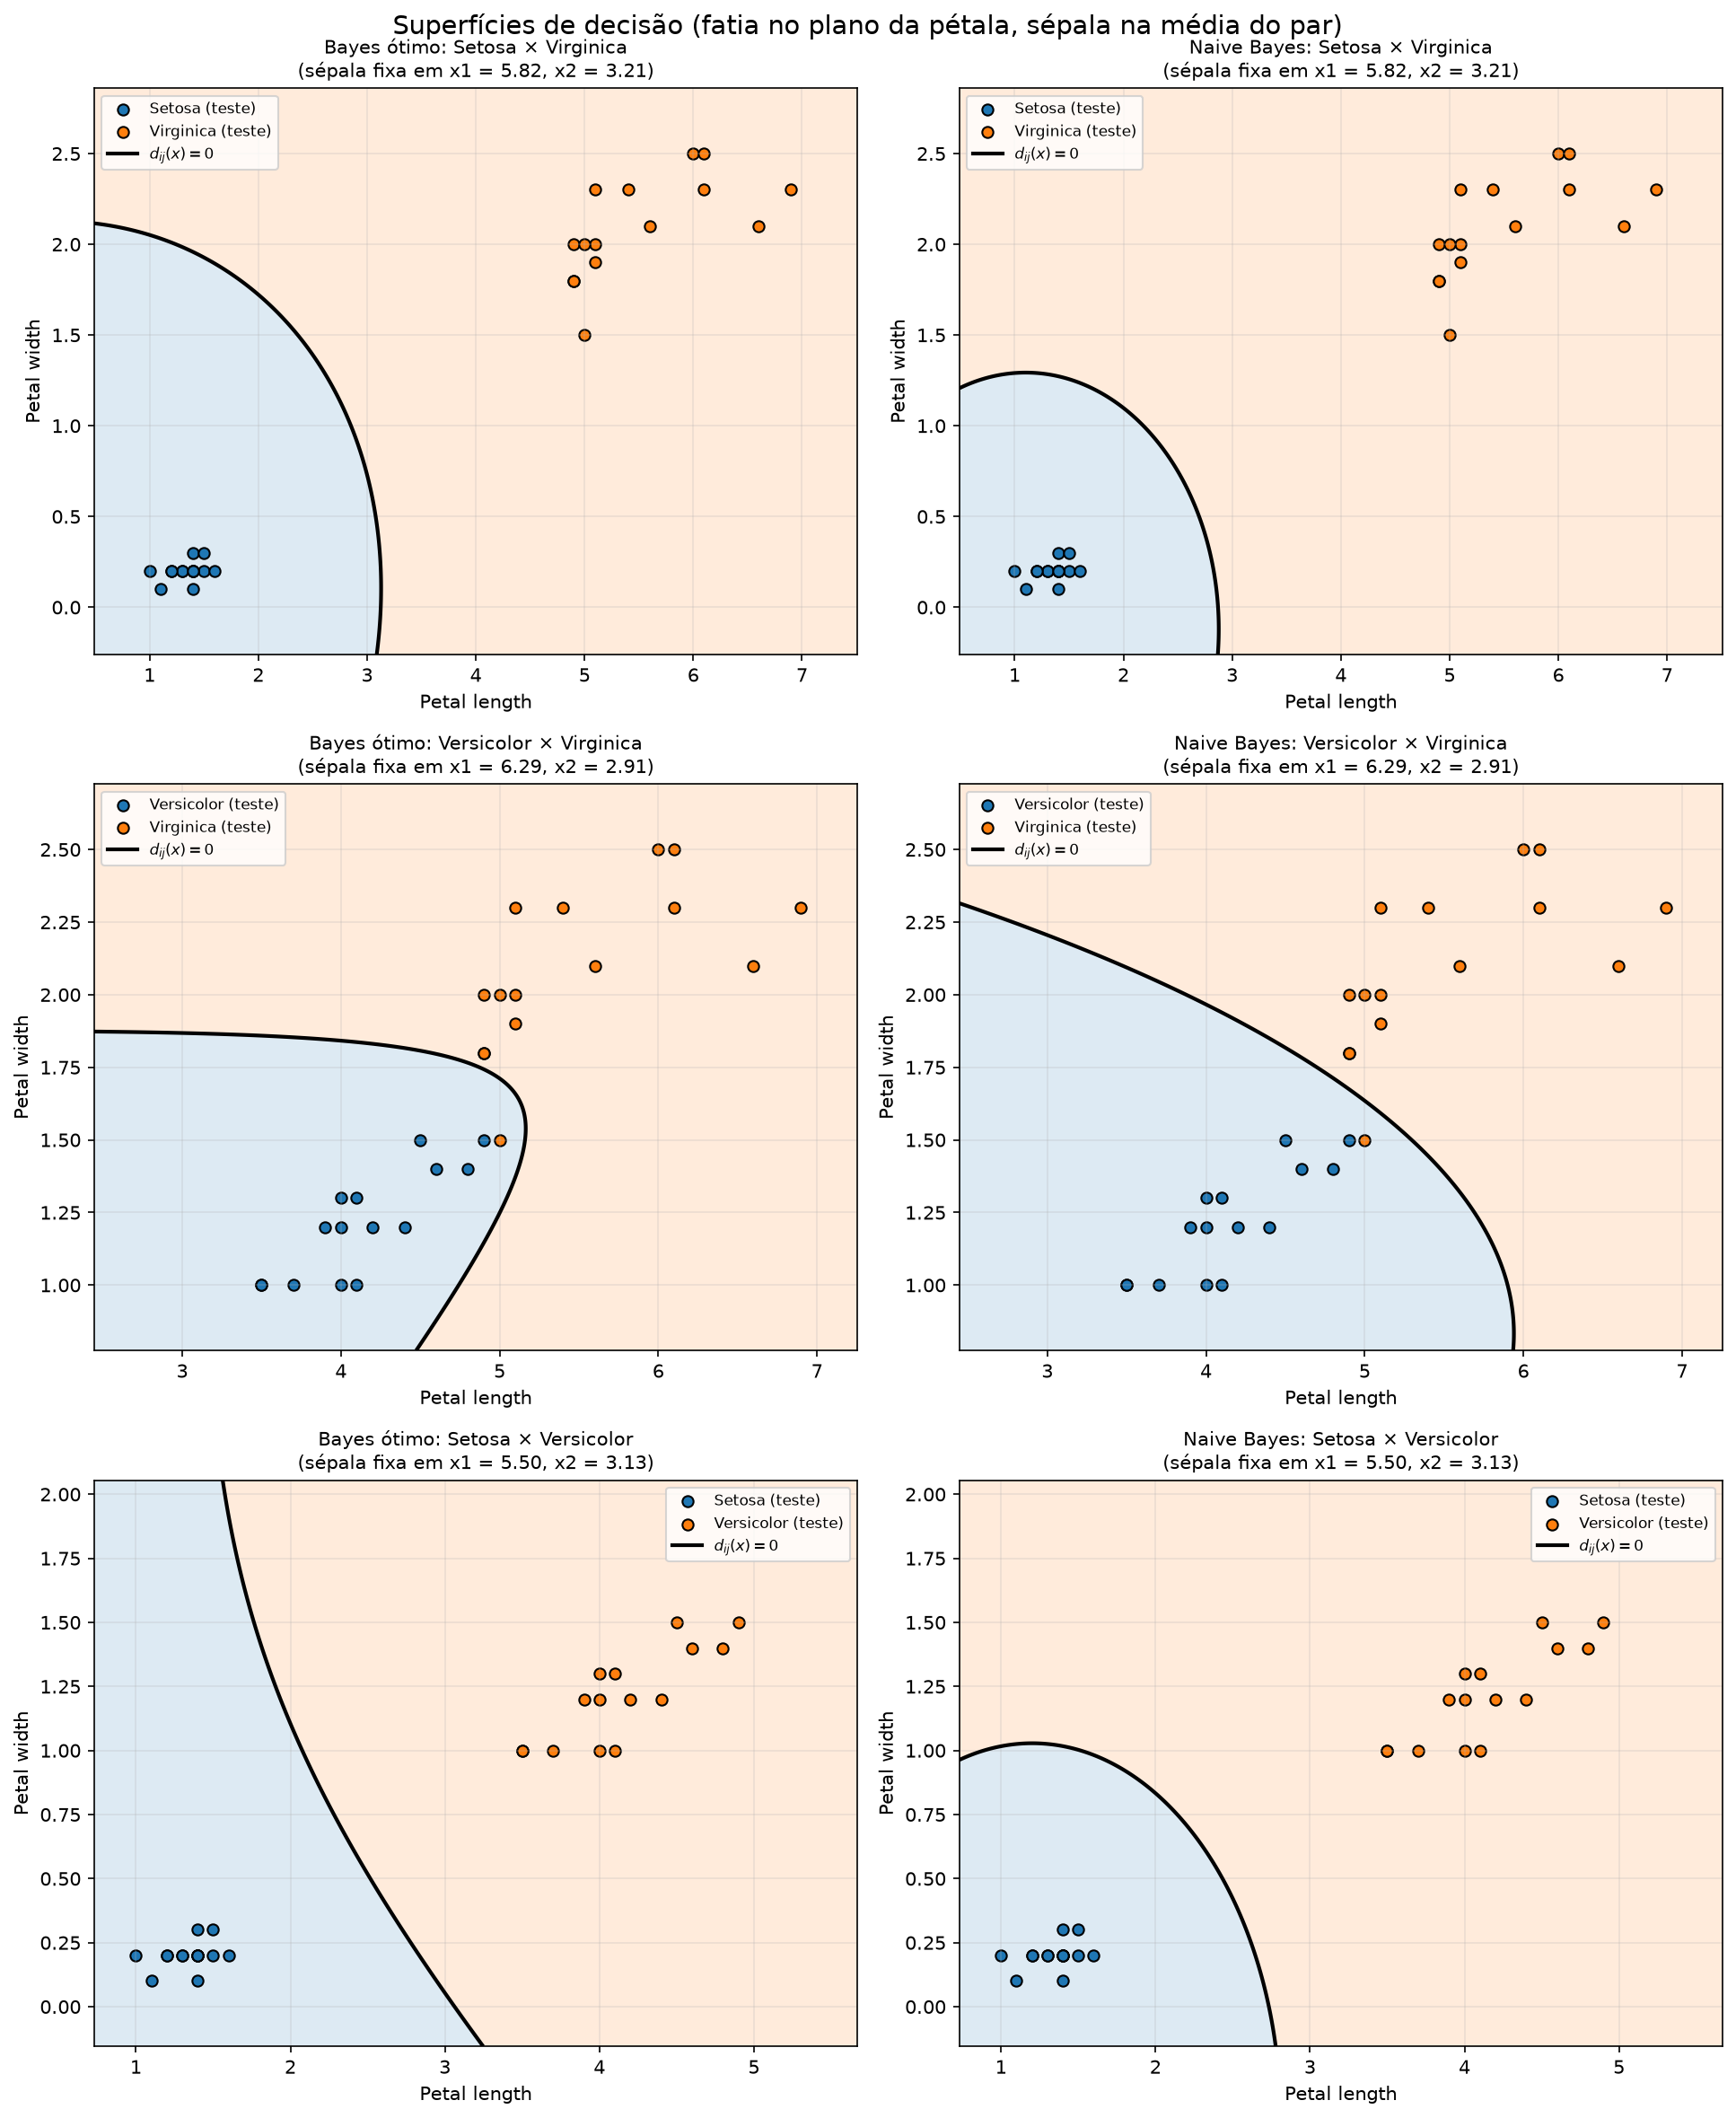
\includegraphics[width=0.92\textwidth]{figuras/superficies_decisao.png}
\caption{Superfícies de decisão no plano da pétala, com as amostras de teste. Coluna da esquerda: classificador ótimo de Bayes; coluna da direita: Naive Bayes.}
\label{fig:superficies}
\end{figure}

Nos pares com a \setosa{}, as regiões da \setosa{} são elipses fechadas em torno da sua nuvem, muito menor que as das outras espécies, e as duas classes ficam bem separadas. No par \versicolor{}~$\times$~\virginica{}, a fronteira do classificador ótimo de Bayes é curvada e se inclina conforme a correlação entre comprimento e largura da pétala, enquanto a do Naive Bayes tem eixos alinhados aos atributos. A fatia é apenas uma visualização: no gráfico do classificador ótimo de Bayes, a \virginica{} de teste em $(x_3, x_4) = (5{,}0;\ 1{,}5)$ aparece do lado da \versicolor{}, mas, com os quatro atributos, ela é classificada corretamente, porque sua sépala não é a média usada no corte.

\subsection{Pares de classes}

\begin{table}[H]
\centering
\caption{Métricas nos pares de classes (teste, 30 amostras por par). A primeira classe do par é a positiva.}
\label{tab:pares}
\small
\begin{tabular}{llrrrrcccccc}
\toprule
Par & Classificador & VP & FP & FN & VN & $A_g$ & $K$ & $\sigma_K^2$ & $F_1$ & $F_2$ & MCC \\
\midrule
\multirow{2}{*}{Set. $\times$ Vir.} & Bayes ótimo & 15 & 0 & 0 & 15 & 1,0000 & 1,0000 & 0 & 1,0000 & 1,0000 & 1,0000 \\
                                    & Naive Bayes & 15 & 0 & 0 & 15 & 1,0000 & 1,0000 & 0 & 1,0000 & 1,0000 & 1,0000 \\
\midrule
\multirow{2}{*}{Ver. $\times$ Vir.} & Bayes ótimo & 15 & 0 & 0 & 15 & 1,0000 & 1,0000 & 0 & 1,0000 & 1,0000 & 1,0000 \\
                                    & Naive Bayes & 15 & 1 & 0 & 14 & 0,9667 & 0,9333 & 0,004277 & 0,9677 & 0,9868 & 0,9354 \\
\midrule
\multirow{2}{*}{Set. $\times$ Ver.} & Bayes ótimo & 15 & 0 & 0 & 15 & 1,0000 & 1,0000 & 0 & 1,0000 & 1,0000 & 1,0000 \\
                                    & Naive Bayes & 15 & 0 & 0 & 15 & 1,0000 & 1,0000 & 0 & 1,0000 & 1,0000 & 1,0000 \\
\bottomrule
\end{tabular}
\end{table}

Os pares com a \setosa{} são classificados sem erro pelos dois métodos. Em \versicolor{}~$\times$~\virginica{}, o Naive Bayes repete o erro da classificação das três classes (sensibilidade da \virginica{} 0,9333, especificidade 0,9333 para a \versicolor{}), e o classificador ótimo de Bayes acerta tudo.

\subsection{Teste de significância}\label{sec:teste}

\begin{table}[H]
\centering
\caption{Item (e): classificador ótimo de Bayes vs.\ Naive Bayes nas três classes ($\alpha = 5\%$).}
\label{tab:teste}
\begin{tabular}{lccccc}
\toprule
Coeficiente & Bayes ótimo & Naive Bayes & $Z$ & p-valor & Decisão \\
\midrule
Kappa & 1,0000 & 0,9667 & 1,0121 & 0,3115 & não rejeita $H_0$ \\
Tau   & 1,0000 & 0,9667 & 1,0113 & 0,3119 & não rejeita $H_0$ \\
\bottomrule
\end{tabular}
\end{table}

O classificador ótimo de Bayes tem a maior acurácia (100\% contra 97,78\%), mas $|Z| = 1{,}01 < 1{,}96$ e $p = 0{,}31$: não se rejeita $H_0$, e a diferença não é estatisticamente significativa ao nível de 5\%. Se os dois classificadores fossem equivalentes, uma diferença de Kappa pelo menos desse tamanho apareceria por acaso em cerca de 31\% das amostras de teste. Como o Kappa do classificador ótimo de Bayes é 1, sua variância é nula, e o denominador da Eq.~\eqref{eq:z} vem apenas da variância do Naive Bayes.

\paragraph{Sensibilidade à divisão.} Para avaliar o quanto o resultado depende da divisão 70/30, o experimento foi repetido com as sementes 0 a 9 (Tabela~\ref{tab:sementes}). O classificador ótimo de Bayes teve acerto maior em 5 divisões, empatou em 4 e perdeu em 1, e nenhuma diferença foi significativa.

\begin{table}[H]
\centering
\caption{Acerto global e teste $Z$ do Kappa em 10 divisões 70/30.}
\label{tab:sementes}
\small
\begin{tabular}{ccccccc}
\toprule
Semente & $A_g$ Bayes & $A_g$ Naive & $K$ Bayes & $K$ Naive & $Z$ & $p$ \\
\midrule
0 & 1,0000 & 1,0000 & 1,0000 & 1,0000 & 0,000      & 1,000 \\
1 & 0,9111 & 0,9333 & 0,8667 & 0,9000 & $-0{,}395$ & 0,693 \\
2 & 0,9556 & 0,9333 & 0,9333 & 0,9000 & 0,462      & 0,644 \\
3 & 0,9778 & 0,9778 & 0,9667 & 0,9667 & 0,000      & 1,000 \\
4 & 0,9333 & 0,9333 & 0,9000 & 0,9000 & 0,000      & 1,000 \\
5 & 0,9778 & 0,9556 & 0,9667 & 0,9333 & 0,590      & 0,555 \\
6 & 0,9556 & 0,9556 & 0,9333 & 0,9333 & 0,000      & 1,000 \\
7 & 0,9778 & 0,9556 & 0,9667 & 0,9333 & 0,588      & 0,556 \\
8 & 0,9778 & 0,9556 & 0,9667 & 0,9333 & 0,588      & 0,556 \\
9 & 1,0000 & 0,9778 & 1,0000 & 0,9667 & 1,012      & 0,312 \\
\bottomrule
\end{tabular}
\end{table}

%=====================================================================
\section{Discussão}
%=====================================================================

Os dois classificadores têm desempenho muito alto na Iris, o que é esperado: com densidades normais e covariâncias próprias para cada classe, as fronteiras quadráticas se ajustam melhor à forma das nuvens do que as fronteiras lineares dos laboratórios anteriores. A \setosa{}, linearmente separável das outras espécies, não oferece dificuldade a nenhum método. Todos os erros, quando existem, estão entre \versicolor{} e \virginica{}, cujas nuvens se sobrepõem.

A diferença entre os dois métodos está nas correlações entre atributos. Na \versicolor{} e na \virginica{}, os comprimentos da sépala e da pétala têm correlação alta, e as fronteiras do classificador ótimo de Bayes acompanham essa inclinação (Figura~\ref{fig:superficies}). O Naive Bayes, ao supor independência, só consegue produzir fronteiras com eixos alinhados aos atributos. O preço do modelo completo é estimar 14 parâmetros por classe, contra 8 do Naive Bayes, a partir de 35 amostras; com bases menores ou com mais atributos, essa estimativa ficaria instável, e o Naive Bayes poderia ser a melhor opção.

A hipótese de normalidade foi bem sustentada para \versicolor{} e \virginica{} e é aproximada para a \setosa{}. O resultado do Henze-Zirkler para a \setosa{} mostra a importância de examinar o p-valor com precisão suficiente: arredondado para três casas, ele aparece como 0,05, e a decisão pelo critério $p > 0{,}05$ fica ambígua. Na prática, a aproximação não prejudica a classificação, porque a \setosa{} está muito afastada das outras classes, e qualquer modelo razoável de sua densidade leva à mesma decisão.

Por fim, o teste de significância mostra que a vantagem do classificador ótimo de Bayes, embora consistente (ele foi melhor ou igual ao Naive Bayes em 9 das 10 divisões), não é estatisticamente comprovada com 45 amostras de teste: cada erro muda o acerto global em 2,2 pontos percentuais, e um único erro de diferença está longe de ser significativo. O teste $Z$ também supõe matrizes independentes, mas os dois classificadores foram avaliados nas mesmas amostras, o que torna o teste conservador.

%=====================================================================
\section{Conclusão}
%=====================================================================

O classificador ótimo de Bayes e o Naive Bayes foram implementados sem bibliotecas de aprendizado de máquina, com densidades normais e regra de decisão pelo máximo a posteriori com probabilidades a priori iguais. A aderência à normal multivariada foi verificada pelos testes de Henze-Zirkler e de Mardia, no R e em uma implementação própria em Python, com resultados idênticos: \versicolor{} e \virginica{} são compatíveis com a normal multivariada, e a \setosa{} é limítrofe, rejeitada pelo Henze-Zirkler por margem mínima ($p = 0{,}04995$) e aceita pelos testes de Mardia.

Com 70\% das amostras para treinamento e 30\% para teste, o classificador ótimo de Bayes acertou todas as 45 amostras de teste ($A_g = 1$, $K = \tau = 1$), e o Naive Bayes errou uma \virginica{} ($A_g = 0{,}9778$, $K = \tau = 0{,}9667$). As superfícies de decisão dos três pares foram determinadas analiticamente: são quádricas com termos cruzados no classificador ótimo de Bayes e quádricas sem termos cruzados no Naive Bayes. Nos pares, os dois métodos separam a \setosa{} sem erro, e só o Naive Bayes erra em \versicolor{}~$\times$~\virginica{}.

O classificador ótimo de Bayes tem a maior acurácia, mas, pelo teste de significância do Kappa ($Z = 1{,}012$, $p = 0{,}312$) e do Tau ($Z = 1{,}011$, $p = 0{,}312$), a diferença não é estatisticamente significativa ao nível de 5\%.

%=====================================================================
% Referências
%=====================================================================
\begin{thebibliography}{9}

\bibitem{sousa5}
SOUSA, R. P. de. \textbf{Classificador ótimo de Bayes e Naive Bayes}. Material didático da disciplina Tópicos Especiais em Inteligência Artificial (PR5). Campina Grande: Universidade Estadual da Paraíba, 2026.

\bibitem{sousa51}
SOUSA, R. P. de. \textbf{Métricas de qualidade: machine learning --- aplicações em saúde e diagnóstico clínico}. Material didático da disciplina Tópicos Especiais em Inteligência Artificial (PR51). Campina Grande: Universidade Estadual da Paraíba, 2026.

\bibitem{henze}
HENZE, N.; ZIRKLER, B. A class of invariant consistent tests for multivariate normality. \textbf{Communications in Statistics --- Theory and Methods}, v. 19, n. 10, p. 3595--3617, 1990.

\bibitem{mardia}
MARDIA, K. V. Measures of multivariate skewness and kurtosis with applications. \textbf{Biometrika}, v. 57, n. 3, p. 519--530, 1970.

\bibitem{mvn}
KORKMAZ, S.; GOKSULUK, D.; ZARARSIZ, G. MVN: an R package for assessing multivariate normality. \textbf{The R Journal}, v. 6, n. 2, p. 151--162, 2014.

\bibitem{duda}
DUDA, R. O.; HART, P. E.; STORK, D. G. \textbf{Pattern Classification}. 2. ed. New York: Wiley, 2001.

\bibitem{congalton}
CONGALTON, R. G.; GREEN, K. \textbf{Assessing the Accuracy of Remotely Sensed Data: Principles and Practices}. 2. ed. Boca Raton: CRC Press, 2009.

\bibitem{repo}
PAMPLONA, J. \textbf{Laboratório 04: classificador ótimo de Bayes e Naive Bayes aplicados à base Iris}. Repositório de código-fonte, 2026. Disponível em: \repositorio. Acesso em: nov. 2026.

\end{thebibliography}

\end{document}
